\begin{anexosenv}
% Imprime uma página indicando o início dos anexos
\partanexos

\chapter{Arquitetura do modelo Rafael-2}
\begin{figure}[htb]
	\begin{center}
		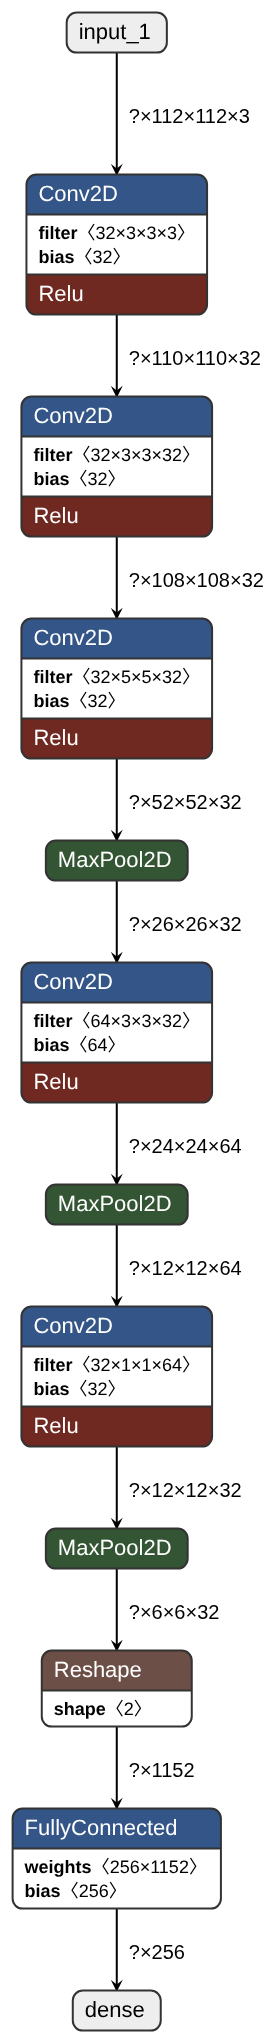
\includegraphics[scale=0.25]{Imagens/rafael_student_r8g8b8_tflite}
	\end{center}
	\caption {Arquitetura do modelo Rafael-2} \legend {Fonte: Autor}
\end{figure}
%
% \begin{center}
% \begin{table}[htb]
% \centering
% \ABNTEXfontereduzida
% \caption[Acurácia dos modelos]{Acurácia dos modelos.}
% \begin{tabular}{ |c|c|c|c| }
% 	% Fonte: https://www.seeedstudio.com/blog/2019/10/24/microcontrollers-for-machine-learning-and-ai/
% 	\hline
% 	\textbf{CPU (Clock Speed)} 	& \textbf{RAM}  & \textbf{Preço} & \textbf{Link} \\
% 	\hline
% 	Quad-core Cortex-A53 (2.30GHz)	& 1GB		& \$129.99	 & https://www.seeedstudio.com/Coral-Dev-Board-p-2900.html \\
% 	Quad-core ARM A57 (1.43GHz) 	& 4GB		& \$89.00	 & https://www.seeedstudio.com/NVIDIAr-Jetson-Nanotm-Developer-Kit-p-2916.html \\
% 	RISC-V Dual Core (400Mhz)  	& 8MB		& \$40.90	 & https://www.seeedstudio.com/Sipeed-MAix-GO-Suit-for-RISC-V-AI-IoT-p-2874.html \\
% 	Cortex-A72 - ARM v8 (1.5GHz)	& 1GB 		& \$35.90	 & https://www.seeedstudio.com/Raspberry-Pi-4-Computer-Model-B-1GB-p-4078.html \\
%
% 	\hline
% \end{tabular}
% \legend{Fonte: Autor}
% \end{table}
% \end{center}
%
% % % ---
% % \chapter{Morbi ultrices rutrum lorem.}
% % % ---
% % \lipsum[30]
% %
% % % ---
% % \chapter{Cras non urna sed feugiat cum sociis natoque penatibus et magnis dis
% % parturient montes nascetur ridiculus mus}
% % % ---
% %
% % \lipsum[31]
% %
% % % ---
% % \chapter{Fusce facilisis lacinia dui}
% % % ---
% %
% % \lipsum[32]
%
%
\end{anexosenv}
